\documentclass[preprint]{sigplanconf}
%\documentclass{sig-alternate}
\usepackage{epsfig, times, graphicx, amssymb, amsmath, amsfonts}

\newcommand{\mt}[1]{\mbox{\it #1}}

\begin{document}

\conferenceinfo{LCTES'05,} {June 15--17, 2005, Chicago, Illinois, USA.}
\CopyrightYear{2005}
\copyrightdata{1-59593-018-3/05/0006} 

\title{Cache Aware Optimization of Stream Programs}
\authorinfo{Janis Sermulins \and William Thies \and Rodric Rabbah \and Saman Amarasinghe}
	     {Computer Science and Artificial Intelligence Laboratory, Massachusetts Institute of Technology}
	     {\{janiss, thies, rabbah, saman\}@csail.mit.edu}

\maketitle

\begin{abstract}
Due to the high data rates involved in audio, video, and signal
processing applications, it is imperative to compress the data to
decrease the amount of storage used.  Unfortunately, this implies that
any program operating on the data needs to be wrapped by a
decompression and re-compression stage.  Re-compression can incur
significant computational overhead, while decompression swamps the
application with the original volume of data.

In this paper, we present a program transformation that greatly
accelerates the processing of compressible data.  Given a program that
operates on uncompressed data, we output an equivalent program that
operates directly on the compressed format.  Our transformation
applies to stream programs, a restricted but useful class of
applications with regular communication and computation patterns.  Our
formulation is based on LZ77, a lossless compression algorithm
utilized by ZIP, and immediately applies to simpler formats such as
Apple Animation, Microsoft RLE, and Targa.

We implemented a simple subset of our techniques in the StreamIt
compiler, which emits executable plugins for two popular video editing
tools: MEncoder and Blender.  For common operations such as color
adjustment and video compositing, computing directly on compressed
data offers a speedup roughly proportional to the overall compression
ratio.  For our benchmark suite of 12 videos in Apple Animation
format, speedups range from 1.1x to 471x, with a median of 15x.

\end{abstract}

\category{D.3.4}{Programming Languages}{Processors}[Optimization; code generation; compilers]
\category{D.3.2}{Programming Languages}{Language Classifications}[Concurrent, distributed, and parallel languages; Data-flow languages]
%\category{D.2.2}{Software Engineering}{Software Architectures, Design Tools and Techniques}

\terms 
Languages, Design, Performance

\keywords
Stream Programing, StreamIt, Synchronous Dataflow, Cache, Cache
Optimizations, Fusion, Embedded

\section{Introduction}


Stream computing represents an increasingly important class of
applications. In streaming codes, there is an abundance of parallelism that
is easier to extract compared to traditional desktop workloads (e.g.,
pointer-based computing). As a result, the extraction of parallelism
in streaming codes does not require heroic efforts, and thus,
processors can deliver higher performance with significantly lower
power costs. This is especially important since
leading microprocessor companies have realized that modern general
purpose architectures are near their  performance limits for  the
amount of power they consume. Thus, the future will place a greater
emphasis on exploiting the properties of streaming workloads in
conventional von~Neumann architectures.

Streaming is a model of computation that uses sequences of data
and computation kernels to expose concurrency and locality for
efficiency~\cite{wss}. In general purpose processors, improving locality 
translates to an effective management of the memory hierarchy at all
levels, including the register file. In this paper, we present a
methodology for compiling streaming codes to general purpose,
cache-based architectures. We first introduce a simple model for
reasoning effectively about the caching behavior of streaming
workloads. This model serves as a foundation for several {\it cache-aware
optimizations} that are geared toward the concomitant increase of instruction
and data {\it temporal locality}. These
optimization lead to significantly better utilization of the memory
system, and as such, they deliver performance gains ranging from 11
to 99\% for our streaming benchmark suite.

The context for our work is StreamIt, an architecture-independent
language that is engineered for streaming
applications~\cite{streamitcc}. It adopts the 
Cyclo-Static Dataflow~\cite{BELP96} model of computation which is a
generalization of Synchronous Dataflow~\cite{LM87-i} (SDF).  
SDF is a popular  model that  is well suited for
streaming codes. In SDF, computation is represented as a graph
consisting of {\it  actors} connected by communication channels; the
actors consume  and produce a constant number  of items from their
input and output  channels every time they execute. SDF is appealing
because it is amenable to static scheduling and optimization. 

From a general purpose architecture's point of view, actors represent
computation kernels, and the communication between actors represents
data buffers that must be streamed to and from the processor. Thus
the size of an actor and the
order of actor executions are critical properties that
impact the performance of the instruction cache. For example, the
compiler must make sure the actor's code size is not
greater than the instruction cache. Furthermore, we must {\it scale}
the execution of the actor so that it runs several times before we move
on to some other actor in the stream 
graph. This serves to $(i)$ amortize the cost of fetching the actor's
instructions into the cache from memory (an expensive operation), $(ii)$
improve the instruction temporal locality, and $(iii)$ improve overall
performance. However, as our cache model will show, we 
cannot arbitrarily scale the execution frequency of an actor. This
is because actors produce data that must be buffered, and therefore,
we must also consider the amount of data an actor produces and
consumes if we are to adequately manage the data cache. This paper is unique
in that it is the first to present a unified optimization methodology
that simultaneously considers instruction and data locality for
mapping streaming computation to cache-based architectures.

In terms of improving the data cache behavior, the compiler schedules
actor firing such that the producer-consumer locality is
preserved. Furthermore,  the compiler may {\it fuse}
together two or more actors to form a coarser grained kernel.
The fusion allows for better register allocation as we can
destroy the arrays used to buffer data between the actors and replace
the corresponding array references with scalars.  It also allows for
various competing implementations for managing the buffers between the
fused actors.  This paper evaluates several implementation
alternatives (for buffer management) and evaluates their performance.

The methodology for fusing actors leverages a distinguishing StreamIt
characteristic, namely, the hierarchical organization of
the stream graph. Furthermore, the algorithm for fusing actors applies
for the various topologies allowed by StreamIt.
It also considers another distinguishing characteristics of StreamIt,
namely the {\tt peek} operation whereby an actor may inspect data
items in its input buffer without consuming them until some future
execution. While peeking is a powerful language feature, it does pose
some challenges to the compiler and the cache optimizations. Peeking
also impacts the choice for the best buffer management strategy, as our
study will show.

%% the comment about p3 and itanium not being embedded architectures
%% is out of the blue! need a better transition.
Cache-aware fusion alone delivers significant performance gains, although our
evaluation shows that fusion with scaling leads to the best
performance on a general purpose, cache-based architecture. For our
experiments, we use two different processors: a superscalar out-of-order
processor, and an in-order VLIW processor. The former is a Pentium~3
whereas the latter is an Itanium~2. While these architectures are not
particularly suited for an embedded system, they do exhibit some
properties that are worthy of investigation. Furthermore, that we can
demonstrate measurable performance gains on real systems is far more
convincing than using a simulation-based environment. We chose the
Pentium~3 processor because it has very few registers in its
instruction set architecture. The Itanium by contrast has a much 
larger and richer repertoire of registers. The two architectures serve
to validate our cache-aware optimizations, in that we expect an
architecture with more register to benefit more from optimization such
as scalar replacement. On average, fusion leads to a 47\% improvement
on the Pentium~3, and 50\% on the Itanium~2.

The two architectures also differ in terms of their memory system
organization. The Itanium is an in-order VLIW processor and does not
tolerate a memory stall as well as its out-of-order
counterpart. Therefore we expect different gains from the scaling
optimization which amortize the long access latencies for instruction
and data caches. On average, scaling leads to a 21\% improvement on
the Itanium~2, and 17\% on the Pentium~3.

While both scaling and fusion lead to modest performance gains, we
must combine the two to deliver the best possible performance. When we
do so, we can further improve the performance of our benchmarks by
53\% on average for the Pentium~3, and 55\% for the Itanium~2.

\subsection{Summary of Contributions}

This paper makes the following contributions:
\begin{itemize}

\item A cache model for stream computing that provides a quantitative
estimate of the caching performance for any sequence of actor
executions.

\item A cache-aware scheduling heuristic that judiciously increases
the multiplicity of actors, improving instruction and data locality
while not exceeding the data cache.

\item A cache-aware partitioning policy that judiciously fuses
adjacent actors into a single component, enabling local optimizations
while not exceeding the instruction cache.

\item An optimized buffer management policy, termed ``copy-shift with
execution scaling'', which out-performs a traditional rotating buffer
in a detailed micro-benchmark analysis.

\item A fully automatic implementation of the above techniques in the
StreamIt compiler.

\item An experimental evaluation across 11 streaming benchmarks,
demonstrating performance improvements of up to 99\%.
\end{itemize}

\subsection{Paper Roadmap}

The remainder of the paper is organized as follows. Section~\ref{sec:streamit}
describes StreamIt and introduces our motivating example.
Section~\ref{sec:cache-model} introduces our cache model for 
reasoning about the performance of a streaming
computation. Section~\ref{sec:cache-opt} describes our cache-aware
optimizations, and Section~\ref{sec:buffer} describes the 
optimization enabled by fusion. Section~\ref{sec:evaluation} describes
our evaluation methodology and present our experimental
analysis. Sections~\ref{sec:related-work}~and~\ref{sec:conclusion}
discuss related work and concludes the paper.

\section{StreamIt}
\label{sec:streamit}

StreamIt  is   an  architecture-independent  language that was
designed for  streaming applications. In StreamIt, programs are
represented as graphs where  nodes represent  computation and edges
represent FIFO-ordered communication of data over tapes.

The  basic programmable  unit (i.e., an actor) in  StreamIt is a {\it
filter}.   Each filter contains  a work  function that executes
atomically,  popping (i.e., reading)  a fixed number  of items  from
the  filter's input  tape and pushing (i.e., writing) a fixed number
of items to the filter's output tape.  A filter  may also {\tt peek} at
a given index  on its input tape without  consuming  the  item;  this
makes  it  simple  to  represent computation over a
sliding-window.   The {\tt push}, {\tt pop}, and {\tt peek} rates are
declared as part  of  the work  function,  thereby enabling  the
compiler    to construct a static schedule of filter executions. The
following is an example implementation of a FIR   (Finite Impulse
Response)  filter: 
%\begin{scriptsize}
{\small
\begin{verbatim}
float->float filter FIR (int N, float[] weights) 
{
  work push 1 pop 1 peek N {
    float sum = 0;
    for (int i = 0; i < N; i++) {
      sum += peek(i) * weights[i];
    }
    pop();
    push(sum);
  }
}
\end{verbatim}}
%\end{scriptsize}

The work function is invoked (fired) whenever there is sufficient data
on the input tape. In this case, the filter requires at least
\texttt{N} elements before it can execute. The value of \texttt{N} is
known at compile time when the filter is composed to form a stream
graph. A filter is akin to a class in object oriented programming
with the work function serving as the main method. The parameters
to a filter (e.g., \texttt{N} and \texttt{weights}) are equivalent to
parameters passed to a class constructor. In StreamIt, the
application developer focuses on the hierarchical assembly of the
stream graph and its communication topology, rather than on the 
explicit management of the data buffers between filters.

\begin{figure}[t]
\begin{center}
\vspace{-24pt}
 \framebox{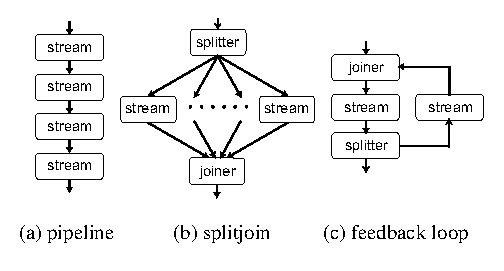
\includegraphics[scale=1, angle=0]{./constructs-eg.eps}}
 \vspace{-6pt}
 \caption{StreamIt containers.}
 \label{fig:containers}
\end{center}
\end{figure}

\begin{figure}[t]
\begin{center}
\vspace{-12pt}
 \framebox{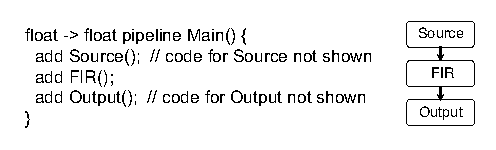
\includegraphics[scale=1, angle=0]{./pipeline-eg.eps}}
 \vspace{-6pt}
 \caption{Example pipeline with FIR filter.}
 \label{fig:pipeline}
\vspace{-18pt}
\end{center}
\end{figure}

StreamIt provides three hierarchical structures for composing filters
into larger stream graphs (see Figure~\ref{fig:containers}). The 
{\it pipeline} construct composes streams in sequence, with the output
of one connected to the input of the next.   An example of a pipeline
appears in Figure~\ref{fig:pipeline}.

The {\it splitjoin} construct distributes data to a set of parallel
streams, which are then joined together in a round robin fashion.  In
a splitjoin, the {\it splitter} performs the data scattering, and the
{\it joiner} performs the gathering. A splitter is a specialized
filter with a single input and  multiple output channels. On 
every execution step, it can distribute its output to any one of
its children in either a {\it duplicate} or a {\it roundrobin}
manner. For the former, incoming data is replicated to every
sibling connected to the splitter. For the latter, data is scattered
in a round-robin manner, with each item sent to exactly one child
stream, in order.  The splitter type and the weights for distributing data to
child streams are declared as part of the syntax (e.g., \texttt{split
duplicate} or \texttt{split roundrobin($w_0$, $w_1$, ... $w_n$)}). The
splitter counterpart, the joiner, is a specialized filter with  
multiple input channels but only one output channel. The joiner
gathers data from its predecessors in a round-robin manner (declared
as part of the syntax). 

StreamIt also provides a {\it feedback loop} construct for introducing
cycles in the graph.

\section{Execution Model}
\label{sec:execmodel}

A StreamIt program is represented by a hierarchical graph,
where the leaf nodes are filters, splitters, and joiners, and
the composite nodes are pipelines, splitjoins, and
feedback-loops. Edges in the graph represent data channels, which 
operate as FIFO queues.
In order for an actor  (i.e., a filter,
splitter, or joiner) to execute, it must have enough data items on its input
tape. In StreamIt, actors have  two epochs
of execution: one for initialization, and one for the steady
state. The initialization primes the input tapes to allow filters with
peeking to execute the very first instance of their work functions;
initialization in this setting is similar to the prologue stage in
software pipelining. The steady state schedule has the property that
the amount of data buffered between any two actors does not change
before and after the actor executions.

\begin{figure}[t]
\begin{center}
\vspace{-24pt}
 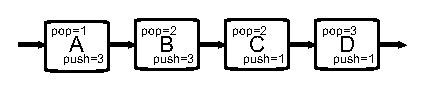
\includegraphics[scale=1, angle=0]{./pipe-with-rates.eps}
\vspace{-6pt}
 \caption{Example pipeline.}
 \label{fig:pipe-with-rates}
\end{center}
\end{figure}

As an example, a steady state schedule for the sample pipeline in
Figure~\ref{fig:pipe-with-rates} requires filter \texttt{A} to fire
four times, \texttt{B} six times, \texttt{C} nine times, and
\texttt{D} three times. 
% Because in StreamIt the filters are
% independent (i.e., they do not share state), they can execute
% concurently. In a uniprocessor setting (which is what we use for our
% evaluation), we can only run one filter at time. Therefore, 
The data generated by one actor is buffered (cached) until it is
consumed.

The StreamIt compiler derives the initialization and steady state
schedules~\cite{karczma-lctes03} and outputs a C program that includes
the initialization and work functions, as well as a driver to execute
each of the two schedules. For example, referring to
Figure~\ref{fig:pipe-with-rates}, the compiler generates the following
sample code for running the steady state schedule:
%\begin{scriptsize}
\begin{verbatim}
run_steady_state() {
  for (i = 0; i < 4; i++) A_work();
  for (i = 0; i < 6; i++) B_work();
  for (i = 0; i < 9; i++) C_work();
  for (i = 0; i < 3; i++) D_work();
}
\end{verbatim}
%\end{scriptsize}
To execute the program, the steady state kernel is wrapped with
another loop that invokes the kernel a designated number of
times. Preceding the state steady, a similar initialization schedule
is run to prime the data buffers, and following the steady state, an
epilogue is run to drain the buffers as necessary.

\begin{figure}[t]
\begin{center}
\vspace{-12pt}
 \psfig{figure=ssi.eps,width=3in}
 \vspace{-6pt}
 \caption{Instruction size (in bytes along the y-axis) per filter
 (x-axis) occurring in a steady state execution of FFT.}
 \label{fig:ssi-single}
\vspace{-18pt}
\end{center}
\end{figure}

From a caching point of view, it is intuitively clear that once a
filter's instruction working set is fetched into the cache, we must
execute that filter as many times as possible to improve instruction
locality and amortize the cost of the accesses to lower levels of the
memory hierarchy. This of course assumes that the total code size for
the filters in the steady state exceeds the capacity of the
instruction cache (which is commonly the case;). In
Figure~\ref{fig:ssi-single} we show a representative breakdown of the
code size per filter in a steady state execution of a StreamIt
implementation of FFT. In all, the total code size for a steady state
ranges from 16~Kb to over 60~Kb for our benchmarks. These results
provide evidence that while individual filters may have a
small instruction footprint, the total footprint of the filters in a
steady state exceeds a typical instruction cache size.
From these observations, it is evident that we must {\it scale} the
execution of filters in the steady state in order to improve temporal
locality. In other words, rather than running a filter $S$ times per
steady state, we increase the loop bound so that it runs $\texttt{M}
\times S$ times (e.g., the loop bound for \verb+A_work+ is
changed to $\texttt{M} \times 4$ in the example shown earlier). 
We term \texttt{M} the {\it multiplicity factor}.

The obvious question is: to what extent can we scale the execution of
filters in the steady state? The answer is non-trivial because
scaling, while beneficial to the instruction cache behavior, may
overburden the data cache as the buffers between actors may grow to
prohibitively large sizes that degrade the data cache
behavior. Specifically, if a buffer overflows the cache, then
produce-consumer locality is lost. 

Also complicating matters is the amount of state a filter must retain
from one execution of its work function to the next. In the FIR
example shown earlier, the filter state is proportional to the size of
the coefficient array (i.e., \texttt{weights}). The filter state
further constrains the schedule scaling.

\section{Cache Model for Streaming}
\label{sec:cache-model}

In this section we describe a simple and intuitve cache model to
estimate the instruction and data cache behavior given an execution
ordering of the filters in the stream graph.

The model is based on the notion of a filter reuse distance which is 
based on LRU stack distance~\cite{mattson70}. We develop the model
first for the instruction cache, and then subsequently generalize it to
account for the data cache.

\subsection{Instruction Cache}

A {\it filter execuion trace} is a sequence of 
filter work functions executions: $T = f_0 f_1 ... f_n$; $f_i$ represents the
execution of filter $f$ at logical time $i$.
The filter {\it instruction reuse distance} ($IRD$) is defined as the
number of unique instructions that are referenced between two
instances of the same work function. Formally, we define $phase(f_i)$
as the sequence $f_i ... f_l$ ($i < l$) of work functions occuring in
$T$ such that $f_i = f_l$ and no where else (i.e., $f_i \neq f_k$
$\forall{k}~~s.t.~~i < k < l$). The $IRD(f_i) = \sum I(f_j)$ over all
distinct filters occuring in $phase(f_i)$, and $I(f)$ equals the code
size of a filter $f$. Based on this reuse metric, we define an
instruction-cache-miss step function $ICM(f_i)$ such that:
\begin{equation}
\label{eq:icm}
  ICM(f_i) =
    \begin{cases}
      0& \text{if $IRD(f_i) \leq C_I$; hit/no cache refill},\\
      1& \text{else; a miss/(some) cache refill}.\\
    \end{cases}
\end{equation}
Note that if $f_i$ is the last occurence of a filter $f$ in the trace,
then $ICM(f_i) = 0$. In Equation~\ref{eq:icm}, $C_I$ represents a
consant proportional to the instruction cache size.

We do not account for the cold start
effects of an execution trace. This does not effect our model, and can
be easily remedied if necessary. To see why this is so, consider the
following two execution traces which represent the executions of work
functions for two filters \texttt{A} and \texttt{B}:
$T_1 = \texttt{A}_1\texttt{A}_2\texttt{B}_3\texttt{B}_4$
and 
$T_2 = \texttt{A}_1\texttt{B}_2\texttt{A}_3\texttt{B}_4$.
In both 
traces, the number of cold starts is the same (i.e., two in all).

What our reuse metric quantifies is the number of misses when a specific work
function is reinvoked. For example, assume that each filter is of the exact
size: $I(\texttt{A}) = I(\texttt{B}) = \lceil{C_I / 2}\rceil + 1$;
that is, the combined instruction workingset of both filters exceeds
the instruction cache, although each filter has a code size that is
smaller than the cache size. Naturally, we expect the trace $T_1$ to
suffer one cold start miss and no other misses for filter \texttt{A}
(and similarly for the other filter). Our model is in accord with
intuition:  $ICM(\texttt{A}_1) = 0$ since
the $IRD(\texttt{A}_1) < C_I$.

In the case of trace $T_2$, we know that since the combined
instruction workingset of the filters exceeds the cache size, when
filter \texttt{B} is invoked following \texttt{A}, it evicts part of
filter \texttt{A}'s instruction workingset. Hence when we transition
back to run filter \texttt{A}, we have to refetch certain
instructions, but in the process, we replace parts of filter
\texttt{B}'s workingset. Hence, we have suffered one cold start miss,
and one capacity miss for filter \texttt{A}, and similarly for
\texttt{B}. Our model is again in accord with intuition: 
$ICM(\texttt{A}_1) = 1$ since
the $IRD(\texttt{A}_1) > C_I$. Note that the
amount of refill is proportional to the number of cache lines that are
replaced when swapping filters, and as such, we may wish to adjust
our cache miss step function. One simple variation is to allow for
some partial replacement without unduly penalizing the overall value
of the metric. Namely, we can allow the constant $C_I$ to be some
fraction greater than the actual cache size. Alternatively, we can use
a more complicated miss function with a more uniform probablity
distribution.

Using the metrics above, we can estimate the instruction-cache miss
rate $(IMR)$ as $\sum ICM(f_i)$ over all $f_i$ in the trace, divided
by the size of the trace. Note that different execution orderings for
the same stream graph lead to traces of the same size and hence the
comparisons are fair. The model allows us to rank the quality of an
execution ordering, with scheduling decisions that boost temporal
locality yielding miss rates closer to zero (and schedules that do not
exploit temporal locality yielding traces with miss rates closer to
one).

Our model predicts that scaling is always beneficial from an
instruction-cache point of view. As a reminder, by scaling, we mean
that a filter's work function is run for a greater number of times in
the steady state before transitioning to the next filter in the
graph. Hence for example, a program that would generate a trace $T_2$
might be as follows:
\begin{verbatim}
run_steady_state() {
  for (i = 0; i < 1; i++) A_work();
  for (i = 0; i < 1; i++) B_work();
}
\end{verbatim}
but a scaled program that increases temporal locality is as follows:
\begin{verbatim}
run_steady_state() {
  for (i = 0; i < M * 1; i++) A_work();
  for (i = 0; i < M * 1; i++) B_work();
}
\end{verbatim}
where \texttt{M} (the multiplicity factor) is an integer greater than
one. From our model, it is easy to see that scaling reduces the number
of misses for a given filter $f$ from $K$ to $\frac{K}{\texttt{M}}- 1$, where $K =
\sum ICM(f)$ for all occurences of $f$ in  the execution trace.

\subsection{Data Cache}

As noted earlier, we can not arbitrarily scale the execution frequency
of a filter wihout also considering how scaling might impact
the data buffer sizes between filers. In this regard, a filter's
output buffer size is also constrained by the amount of state that a
filter retains with every execution of its work function.

Clearly if a filter has any static data (e.g., state information or
coeffecient arrays), then it is prudent to maximize their temporal
access locality. We can define a data-cache miss rate equation ($DMR$) based on
a derivation similar to that for the instruction-cache miss rate:
replace $C_I$ with $C_D$ in Equation~\ref{eq:icm}, and $I(f_i)$ with
$S(f_i)$ when calculating the {\it data reuse distance} ($DRD$). 
Here, $C_D$ represent a constant proportional to the data cache size,
and $S(f)$ represents the total size of the static data in the
specified filter.

The presence of static data in a filter implies that we have to limit
the scaling of a filter $f$ such that it does not require more than $C_D -
S(f_i)$ bytes of buffer space for reading and writing data; otherwise
the data workingset of the filter will overflow the cache and we lose
produce-consumer locality. The buffer requirements are representend by
$Y(f_i)$, and the data-cache model accounts for the dynamic data
requirements by adjusting the data reuse distance as follows:
$DRD(f_i) = \sum (S(f_i) + Y(f_i))$ over all distinct filters occuring
in $phase(f_i)$.

Intuitively, the dynamic data accounts for the size of the buffer
required for writing new values, as well as the size of the buffer
necessary for reading values. It also adjusts for any
producer-consumer locality since the output buffer of one filter is
also the input buffer of its sibling in the stream graph. What this
measures tells us is that we can scale the execution of a filter as
long as its buffer requirements (for reading and writing) do not
exceed the cache, and furthermore, as long as the input-output rates
between producer consumer pairs are not grossly mismatched. This later
qualification is important and motivates a series of cache
optimizations discussed in the next section. In the case of rate
mistmatch, the metric tells us that the effective cache size is
reduced, or in other words, the data that is left over after a
producer-consumer firing must be preserved until a future occurence of
the same pair of filters. This translates to lower data locality and
degrades cache performance.

Mathematically, the dynamic data measure is defined as:
\begin{eqnarray}
  \nonumber
  Y(f_i) &=&\sum_{f_k} min(W(f_k), U(f_k) \times A(f_k)) + \\
  \nonumber
	   &&\sum_{f_k} min(R(f_k), O(f_k) \times A(f_k)) - \\
  \nonumber
         &&\sum_{f_s} O(f_s) \times A(f_s)
\end{eqnarray}
with $W(f)$ equal to the output buffer size reserved for writing data, $R(f)$
equal to the input buffer size reserved for reading data, $U(f)$ equal to the
{\tt push} rate (in bytes) of the filter, $O(f)$ equal to the {\tt pop} rate (in
bytes) of the filter, and $A(f)$ equal to the number of occurences of
filter $f$ in $phase(f_i)$. Also note that the $Y(f_i)$ is defined
over all distinct occurences of $f_k$ in the phase, and $f_s$
represents the filter that comsumes the data produced by $f_k$ (i.e.,
it is $f_k$'s successor in the stream graph, and $f_k$-$f_s$
constitute a producer-consumer pair).

The first term in the equation above quantifies the address space
accessed for writing data. It is  equal to the lesser of the buffer size
reserved for output, and the total number of items produced by
the filter (i.e., the push rate multiplied by the number of times the
work function fired in the phase); this avoid over estimating the
address space when an exceedingly large buffer is reserved but only a
portion of it is used for writing in a phase.

The second term in the equation quantifies the referenced address space 
for reading the input data. This term is also the lesser of two
values: the input buffer size, and the total number of bytes referenced for
reading data.

The third term avoids double counting since the output buffer of one
filter is also the input buffer of its successor in the stream
graph. The term quantifies the amount of data that is consumed by the
producer's successor (which therefore releases a portion of the
address space for use by other filters in the phase).

\subsection{Remarks}

Note  that we can  combine the  instruction and  data cache  miss rate
equations to yield one measure that estimates the temporal locality of
a streaming computation.

Also note that while we use  an execution trace to describe our model,
it  is possible  to  calculate  the instruction  and  data cache  miss
metrics at  compile time.  To do so,  we can leverage  the hiearchical
StreamIt   representation  that  dictates   the  ordering   of  filter
executions.

\section{Cache Optimizations}
\label{sec:cache-opt}

In this section we describe a set of cache-aware transformations that
are geared toward improving the instruction and temporal locality of a
stream graph. We first describe our methodology for scaling actor
firings, and subsequently we describe an optimization that is geared
toward reducing the static and dynamic data requirements of
producer-consumer pairs.

% - multiplicity algorithm
% - forward reference to results

% - partitioning algorithm
% - forward reference to results

\subsection{Multiplicity Scaling}

The goal of this optimization is to increase the execution frequency
of the actors in a steady state schedule, such that the temporal
locality in the memory hierarchy is improved. Our approach is to find a
single multiplicity factor \texttt{M} for scaling all actors, such that
at least 90\% of the actors have a data workingset that fits in the cache.
In other words, using our model, we calculate \texttt{M} such that 
$S(f) + D(f) \leq C_D$
% and $DCM(f) = 0$ % this is wrong!
for 90\% of the actors in the stream graph.

The algorithm 
computes the largest scaling factor for every actor such that its data
workingset does not exceed the size of the primary data cache
(16~Kb on a Pentium~3 for example). This yields a set of multiplicities
${\texttt{M}_0, \ldots, \texttt{M}_n}$ for the actors in the stream
graph. For example, the algorithm might calculate
$\texttt{M}_\texttt{A} = 10$,
$\texttt{M}_\texttt{B} = 20$, 
$\texttt{M}_\texttt{C} = 30$, 
$\texttt{M}_\texttt{D} = 40$ for four filters \texttt{A}, \texttt{B},
\texttt{C}, and \texttt{D} in a stream graph.
The algorithm then examines the
distribution and selects the largest $\texttt{M}_i$
for which 90\% of the actors satisfy our data workingset criterion.
In the example, the 90-10 heuristic
selects $\texttt{M} = 10$, otherwise, the workingset of filter
\texttt{A} will exceed the cache. By contrast,
a 75-25 heuristic selects $\texttt{M} = 20$, where 75\% of the
data workingsets are smaller than the cache, and the remaining 25\%
overflowing it.

The 90-10 heuristic was determined empirically. We found that
increasing the threshold beyond 90\% leads to marginal
performance gains. The graphs in Figure~\ref{fig:9010} show the
performance (y-axis) of our benchmarks for different values of the multiplicity
factor (x-axis). In each plot, the diamond represents the \texttt{M} chosen via
the 90-10 rule, and the square represents the largest calculated
\texttt{M} (e.g., in the example above, the largest \texttt{M} is 40).

\subsection{Actor Coarsening}

In StreamIt, the computation boundaries (i.e., the granularity of a
filter) are determined by the application developed according to the
most natural representation of an algorithm. When compiling to a
cache-based architecture, the presence of a  large number of filters
can lead to a high overhead in terms of context swapping between work
functions, and buffer management for the shared data between filters.
It is the compiler's role to adjust the granularity of execution such
that actors do not vary significantly in terms of code  or data
workingset size.

We use a greedy partitioning algorithm to find a set of vertical cuts
in a stream graph such that the resulting partitions are more or less
balanced. The algorithm uses code size estimation to quantify the
instruction footprint of a partition, and analyzes the work function
declarations to estimate the data buffer requirements. The algorithm
also considers the amount of static state that is persistent across
filter executions. This approach is similar to that in
\cite{streamit-asplos} with two distinctions. First, the algorithm
only considers vertical fusion (i.e., within a pipeline): horizontal
fusion is not beneficial from  caching perspective, and may not even
be feasible. Second, since the graph partitioning is limited to
vertical cuts, our actor coarsening optimizations employs a greedy
algorithm instead of a dynamic programing methodology; this reduces
compilation time. 

The cache-aware coarsening of actors, which we will also refer to as
cache-aware fusion, greatly impacts performance as
our results in Section~\ref{sec:evaluation} will demonstrate.
\section{Buffer Management}
\label{sec:buffer}

A salient characteristic of stream programs is the use of FIFO
channels to communicate between parallel components.  Such channels
make explicit the communication between filters, allowing execution to
proceed in parallel or out-of-order so long as items are produced
before they are consumed.  FIFO channels also provide a natural
abstraction for the programmer, as complex modules can be assembled
from a set of small, reusable components.  For these reasons, it is
important to optimize the performance of communication channels.  An
efficient implementation enables a high-level abstraction for
composing filters without sacrificing performance.

Buffer management in StreamIt is more involved than some other stream
languages, due to the {\tt peek} operation.  The {\tt peek} operation
allows a filter to access an item on its input channel without
removing the item from the channel (removal is done via the {\tt pop}
operation).  The {\tt peek} functionality is very important for
components such as FIR (Finite Impulse Response) filters that access
data over a sliding window.  Because a given data item is accessed by
multiple iterations of the filter, there must be a persistent buffer
that stores items across executions.  In the context of a
uniprocessor, efficient buffer management translates to efficient
maintenance and addressing of this buffer in memory.  On a parallel
system, buffers can also be implemented using network links.

\begin{figure*}[t]
\begin{minipage}{1.7in}
\centering
\psfig{figure=fusion-pipeline.eps,width=0.7in}

\caption{Stream graph for a synthetic buffer test.\protect\label{fig:code-graph}}
\end{minipage}
\hspace{0.3in}
\begin{minipage}{2.2in}
\centering
{\scriptsize
\begin{verbatim}
void->void pipeline BufferTest {
  add Source();
  add FIR();
}

void->float filter Source {
  work push 1 {
    push(random());
  }
}

float->void filter FIR {
  int PEEK = 4;
  work pop 1 peek PEEK {
    float result = 0;
    for (int i=1; i<PEEK; i++) {
      result += i*peek(i);
    }
    pop();
    print(result);
  }
}
\end{verbatim}}

\caption{Original StreamIt code for the buffer test.\protect\label{fig:code-orig}}
\end{minipage}
\hspace{0.3in}
%
\begin{minipage}{2.2in}
\centering
%% modulation
{\scriptsize
\begin{verbatim}
void->void filter BufferTest {
  int PEEK = 4;
  float[4] BUFFER;
  int push_index = 0;
  int pop_index = 0;

  prework {
    for (int i=0; i<PEEK-1; i++) {
      BUFFER[push_index++] = random();
    }
  }

  work {
    // run Source
    BUFFER[push_index] = random();
    push_index = (push_index + 1) & 3;
    
    // run FIR
    float result = 0;
    for (int i=1; i<PEEK; i++) {
      result += i*BUFFER[(pop_index + i) & 3];
    }
    pop_index = (pop_index + 1) & 3;
    print(result);
  }
}
\end{verbatim}}

\caption{Fused buffer test using modulation buffer management strategy.\protect\label{fig:code-modulation}}
\end{minipage}
\vspace{6pt}
\hrule
\end{figure*}


In this section, we explore two basic strategies for buffer management
in stream programs.  The first strategy, termed {\it modulation},
implements a traditional circular buffer that is indexed by wraparound
head and tail pointers.  The second strategy, termed {\it copy-shift},
is a new approach that elides modulo operations by shifting the buffer
contents after each operation.  We demonstrate that, while a naive
implementation of copy-shift can be up to 2X slower than modulation,
optimizations that utilize execution scaling can boost the performance
of copy-shift to be roughly 50\% faster than modulation.

Our study is done in the context of a synthetic benchmark, shown in
Figure~\ref{fig:code-orig}.  As depicted in
Figure~\ref{fig:code-graph}, the benchmark is a pipeline consisting of
a simple source and an FIR filter.  On each iteration, the source
pushes a single item.  The FIR filter calculates a weighted sum over
{\tt PEEK} items of the input, then pops a single item from the
channel.  In our experiments, we vary the {\tt PEEK} value from 1 to
121 items.

\subsection{Modulation}

Figure~\ref{fig:code-modulation} illustrates a fused version of the
benchmark using modulation for buffer management.  For simplicity, we
illustrate each buffer management strategy as a source-to-source
transformation in StreamIt.  Each fused filter contains a {\tt
prework} function in which the source filter executes several times to
prime the communication channel with initial items, as well as a {\tt
work} function that represents the steady-state execution.

The modulation scheme uses a traditional circular-buffer approach.
Three variables are introduced: a {\tt BUFFER} to hold all items
transfered between the filters, a {\tt push\_index} to indicate the
buffer location that will be written next, and a {\tt pop\_index} to
indicate the buffer location that will be read next (i.e., the
location corresponding to {\tt peek(0)}).  The communication
primitives are translated as follows: {\small
\begin{verbatim}
push(val); ==>  BUFFER[push_index] = val;
                push_index = (push_index + 1) % BUF_SIZE;

pop();     ==>  pop_index = (pop_index + 1) % BUF_SIZE;

peek(i)    ==>  BUFFER[(pop_index + i) % BUF_SIZE]
\end{verbatim}}
\noindent The StreamIt compiler converts the modulo operations to
bitwise-and operations by scaling the buffer to a power of two.  Note
that if there are no {\tt peek} operations, then the buffer will be
empty following each execution of the downstream filter.  In this
case, the indices can be reset to zero at the start of each execution
and the modulo operations can be eliminated.  However, in our example
the FIR filter does perform peeking, so the modulo operations are
needed.

{\bf Experimental setup.}  Figures~\ref{fig:buf-p3}
and~\ref{fig:buf-itanium} illustrate the performance of various buffer
management strategies on a Pentium 3 and an Itanium, respectively.
The figures illustrate the execution time per output for the synthetic
benchmark (Figure~\ref{fig:code-orig}) across a range of {\tt PEEK}
values.  Performance is normalized to the modulation strategy with
{\tt PEEK=1}.  To ensure a fair comparison with the scalar replacement
optimization (Section~\ref{sec:scalar-replacement}), all loops in the
original filter are fully unrolled.

{\bf Evaluation.}  The time required for the modulation strategy
increases linearly with the peek rate.  This is expected, as there is
a constant overhead per peek operation.

\begin{figure*}
\nocaptionrule
\begin{minipage}{2.2in}
\hspace{-0.1in}\psfig{figure=arm-buf.eps,width=2.4in}
\caption{Performance of buffer management strategies on a StrongARM.\protect\label{fig:buf-arm}}
\end{minipage}
\hspace{0.1in}
\begin{minipage}{2.2in}
\hspace{-0.1in}\psfig{figure=p3-buf.eps,width=2.4in}
\caption{Performance of buffer management strategies on a Pentium~3.\protect\label{fig:buf-p3}}
\end{minipage}
\hspace{0.1in}
\begin{minipage}{2.2in}
\hspace{-0.1in}\psfig{figure=i2-buf.eps,width=2.4in}
\caption{Performance of buffer management strategies on an Itanium~2.\protect\label{fig:buf-itanium}}
\end{minipage}
\vspace{18pt}
\hrule
\begin{minipage}[t]{2.25in}
%% copy-shift
{\FusionFig
\begin{verbatim}


void->void filter BufferTest {
  int PEEK = 4;
  float[3] BUFFER;

  prework {
    for (int i=0; i<PEEK-1; i++) {
      BUFFER[i] = ... ;
    }
  }

  work {
    float[4] TEMP_BUFFER;
    int push_index = 3;
    int pop_index = 0;

    // copy from BUFFER to TEMP_BUFFER
    for (int i=0; i<3; i++) {
      TEMP_BUFFER[i] = BUFFER[i];
    }

    // run Source
    TEMP_BUFFER[push_index++] = ... ;
    
    // run FIR
    float result = 0;
    for (int i=1; i<PEEK; i++) {
      result += i*TEMP_BUFFER[pop_index+i];
    }
    pop_index++;
    print(result);

    // copy from TEMP_BUFFER to BUFFER
    for (int i=0; i<3; i++) {
      BUFFER[i] = TEMP_BUFFER[i+1];
    }
  }
}
\end{verbatim}}

\caption{Copy-shift strategy.\protect\label{fig:copy-shift}}
\end{minipage}
~~\vrule~~
\begin{minipage}[t]{2in}
%% copy-shift + scalar-replacement
{\FusionFig
\begin{verbatim}


void->void filter BufferTest {
  int PEEK = 4;
  float[3] BUFFER;

  prework {
    for (int i=0; i<PEEK-1; i++) {
      BUFFER[i] = ... ; 
    }
  }

  work {
    float TEMP_BUFFER_0;
    float TEMP_BUFFER_1;
    float TEMP_BUFFER_2;
    float TEMP_BUFFER_3;

    // copy from BUFFER to TEMP_BUFFER
    TEMP_BUFFER_0 = BUFFER[0];
    TEMP_BUFFER_1 = BUFFER[1];
    TEMP_BUFFER_2 = BUFFER[2];

    // run Source
    TEMP_BUFFER_3 = ... ;
    
    // run FIR
    float result = 0;
    result += 1*TEMP_BUFFER_1;
    result += 2*TEMP_BUFFER_2;
    result += 3*TEMP_BUFFER_3;
    print(result);

    // copy from TEMP_BUFFER to BUFFER
    BUFFER[0] = TEMP_BUFFER_1;
    BUFFER[1] = TEMP_BUFFER_2;
    BUFFER[2] = TEMP_BUFFER_3;
  }
}
\end{verbatim}}

\caption{Copy-shift with scalar-replacement.\protect\label{fig:code-scalar-replace}}
\end{minipage}
~~\vrule~~
\begin{minipage}[t]{2.25in}
%% copy-shift + scaling
{\FusionFig
\begin{verbatim}


void->void filter BufferTest {
  int PEEK = 4;
  float[3] BUFFER;

  prework {
    for (int i=0; i<PEEK-1; i++) {
      BUFFER[i] = ... ;
    }
  }

  work {
    float[32] TEMP_BUFFER;
    int push_index = 3;
    int pop_index = 0;

    // copy from BUFFER to TEMP_BUFFER
    for (int i=0; i<3; i++) {
      TEMP_BUFFER[i] = BUFFER[i];
    }

    // run Source 16 times
    for (int k=0; k<16; k++) {
      TEMP_BUFFER[push_index++] = ... ;
    }
    
    // run FIR 16 times
    for (int k=0; k<16; k++) {
      float result = 0;
      for (int i=1; i<PEEK; i++) {
        result += i*TEMP_BUFFER[pop_index+i];
      }
      pop_index++;
      print(result);
    }
      
    // copy from TEMP_BUFFER to BUFFER
    for (int i=0; i<3; i++) {
      BUFFER[i] = TEMP_BUFFER[i+16];
    }
  }
}
\end{verbatim}}

\caption{Copy-shift with execution scaling.\protect\label{fig:code-scaling}}
\end{minipage}
\end{figure*}


\subsection{Copy-Shift}

The copy-shift strategy, illustrated in Figure~\ref{fig:copy-shift},
is a novel approach that shifts the live items to the front of the
buffer at the beginning of each execution.  Because each execution
starts writing and reading to the buffer at the same location, there
is no need for the indices to wraparound and the modulo operations can
be eliminated.  This savings is compounded by additional optimizations
enabled by the copy-shift approach, as described in the subsequent
sections.

However, the cost of this strategy comes in the copying operations: at
the start of each execution, $(\mbox{\it peek} - \mbox{\it pop})$
items are copied from the persistent {\tt BUFFER} to the beginning of
a local {\tt TEMP\_BUFFER}.  All subsequent operations reference the
{\tt TEMP\_BUFFER}, and the live items are copied back to the {\tt
BUFFER} upon completion.  While these two variables could also be
combined into a single buffer, keeping them separate results in a
smaller live data set when the filter is not executing.

The communication primitives are translated as follows:
{\small
\begin{verbatim}
push(val); ==>  TEMP_BUFFER[push_index] = val;
                push_index = push_index + 1;

pop();     ==>  pop_index = pop_index + 1;

peek(i)    ==>  TEMP_BUFFER[pop_index + i]
\end{verbatim}}
\noindent Compared to the modulation scheme, the copy-shift strategy
references the {\tt TEMP\_BUFFER} and does not perform modulo
operations.

{\bf Evaluation.}  As shown in Figures~\ref{fig:buf-p3}
and~\ref{fig:buf-itanium}, the unoptimized copy-shift strategy is the
slowest strategy that we evaluate.  Though the cost per peek operation
is smaller than the modulation scheme, the copying overhead per
iteration also grows with the peek rate and cancels out any savings;
overall, copy-shift performs up to 2X slower than modulation.  The
following sections describe optimizations that can justify taking the
copy-shift approach.

\subsection{Copy-Shift with Scalar Replacement}
\label{sec:scalar-replacement}

The first optimization enabled the copy-shift scheme is dubbed {\it
scalar replacement}.  In contrast to the modulation scheme, the
copy-shift approach can result in array operations that access the
same location on every execution of the filter.  The idea behind
scalar replacement is to fully unroll the loops in the filter, thereby
resolving each array index to an integer literal.  Then, since each
location is fully resolved at compile time, an $n$-length array can be
replaced by a set of $n$ scalar variables: one for each item in the
buffer.  This transformation is illustrated in
Figure~\ref{fig:code-scalar-replace}.

Scalar replacement offers several performance benefits.  Scalar
variables can be register allocated, and as local variables they are
subject to a range of dataflow optimizations (constant propagation,
copy propagation, dead code elimination, etc.).  Replacing array
operations with scalars also eliminates array index calculations.
Despite these benefits, scalar replacement is nearly impossible to do
in a general-purpose language such as C because array contents might
be aliased with other pointers.  StreamIt arrays represent values that
are independent in memory, thereby facilitating this optimization.

Note that scalar replacement can only be applied when array indicices
can be resolved to compile-time constants.  If there is unpredictable
control flow within a filter, or if the loops are too large to unroll,
then scalar replacement does not apply.

{\bf Evaluation.}  Compared to an unoptimized copy-shift strategy,
Figures~\ref{fig:buf-p3} and~\ref{fig:buf-itanium} illustrate that
scalar replacement offers modest gains on our synthetic benchmark.  On
the Pentium 3, improvements range from 14\% to 26\%, while on the
Itanium, improvements range from 3\% to 38\% (depending on the peek
rate).  We conjecture that scalar replacement is more critical for
small filters that perform only a few operations.  Due to the high
communication-to-computation ratio in such filters, there could be
large gains from register-allocating and copy-propagating the
temporary variables.

\subsection{Copy-Shift with Execution Scaling}

A final optimization of the copy-shift strategy uses execution scaling
to dramatically decrease the overhead associated with copying the
buffer contents on each iteration.  In any filter, the number of items
inspected on one execution that need to be saved for the next
execution is $(\mbox{\it peek} - \mbox{\it pop})$.  This represents
the number of items copied by the copy-shift scheme.  However, this
cost can be amortized by scaling the number of executions of the
downstream filter in the fused code.  By enclosing the body of the
filter in a loop, the $\mbox{\it peek}$ and $\mbox{\it pop}$ rates can
be made arbitrarily large, while $(\mbox{\it peek} - \mbox{\it pop})$
remains constant.

Thus, execution scaling reduces the fraction of time spent copying to
an arbitrarily small level.  In our study, we scale the executions of
a filter until $(\mbox{\it peek} - \mbox{\it pop}) \leq (1/4)
\mbox{\it pop}$.  In the synthetic benchmark, this implies that each
filter body executes 16 times before the buffer contents are shifted.
The code resulting from this transformation is shown in
Figure~\ref{fig:code-scaling}.

Note that due to the large loops introduced by execution scaling, it
cannot be used in combination with scalar replacement.  If the loops
were unrolled to resolve the array indices, there could be a negative
impact on the instruction cache.

{\bf Evaluation.}  As shown in Figure~\ref{fig:buf-p3}, the copy-shift
approach with execution scaling performs significantly better than
modulation on the Pentium 3.  Speedups range from 38\% to 65\%, with a
geometric mean of 52\%.  This makes sense, as each peek operation is
cheaper due to the eliminated modulo operations (implemented as
bitwise-and in the modulation scheme), while the overhead from copying
is reduced to a fraction of the original copy-shift approach.  

The gains are also sizable on the Itanium, as shown in
Figure~\ref{fig:buf-itanium}.  Speedups range from 11\% to 86\% (where
{\tt PEEK=1}), with a geometric mean of 34\%.  Keep in mind that these
are speedups of copy-shift with scaling over modulation; the speedups
over unoptimized copy-shift are even greater.

\subsection{Summary}

We conclude that copy-shift with execution scaling is the best buffer
management strategy for filters that utilize peeking.  This is
somewhat surprising because the unoptimized copy-shift strategy has
large overheads that result in a slowdown relative to a circular
buffer with modulation.  However, by leveraging the flexibility of the
parallel stream graph to perform execution scaling, the overheads are
amortized and there are significant speedups (geometric means of 52\%
on the P3 and 34\% on the Itanium) over a plain circular buffer
strategy.

%% \subsection{Reusing Intermediate Storage Variables}

%% Once loops have been unrolled, filters have been fused into a
%% partition and arrays have been replaced with scalar variables we can
%% find approximations of live ranges for the new variables and use this
%% information to reduce stack space required by the partition's work
%% function.

%% We replace the scalar variables that have been created as a result of
%% destroying arrays with a minimal number of variables, where minimal
%% number is the maximum number of overlapping live ranges at any point
%% in the work function of the fused partition.

%% The above optimization improves data access locality.

\section{Experimental Evaluation}
\label{sec:evaluation}

\begin{table}[t]
\center
\label{tab:benchmarks}
\vspace{-12pt}
{\tiny
\begin{tabular}{|c|c|c|} \hline
{\bf benchmark}&{\bf description}&{\bf \# of actors}\\ \hline \hline
\texttt{bitonic	} &bitonic sort of 64 integers	&	972 \\ \hline
\texttt{fir	      } &finite impulse response program	&	132 \\ \hline
\texttt{fft-fine	} &fine grained FFT implementation	&	267 \\ \hline
\texttt{fft-coarse} &coarse grained FFT implementation	&	26 \\ \hline
\texttt{3gpp	} &3GPP Radio Access Protocol application	&	105 \\ \hline
\texttt{beamformer} &beamformer with 64 sources and 1 detector& 197 \\ \hline
\texttt{matmult	} &matrix multiplication	&	48 \\ \hline
\texttt{fmradio	} &FM Radio with 10 way equalizer	&	49 \\ \hline
\texttt{filterbank} &simple filterbank program	&	53 \\ \hline
\texttt{filterbank2}&alternate implementation of a filterbank &	37 \\ \hline
\texttt{ofdm	 }& Orthogonal Frequency Division Multiplexor~\cite{spectrumware}	&	16 \\ \hline
\end{tabular}
}
\vspace{-12pt}
\caption{Evaluation benchmark suite.}
\end{table}



\begin{figure*}
\begin{minipage}{3.4in}
\psfig{figure=arm2.eps,width=3.4in}
\caption{Performance of various compilation strategies on a StrongARM.\protect\label{fig:arm-perf2}}
\end{minipage}
\hspace{0.1in}
\begin{minipage}{3.4in}
\psfig{figure=arm1.eps,width=3.4in}
\caption{Full fusion versus \texttt{CAF+scaling+buffer} on a StrongARM.\protect\label{fig:arm-perf}}
\end{minipage}
\end{figure*}

\begin{figure*}
\begin{minipage}{3.4in}
\psfig{figure=p3-2.eps,width=3.4in}
\caption{Performance of various compilation strategies on a Pentium~3.\protect\label{fig:p3-perf2}}
\end{minipage}
\hspace{0.1in}
\begin{minipage}{3.4in}
\psfig{figure=p3-1.eps,width=3.4in}
\caption{Full fusion versus \texttt{CAF+scaling+buffer} on a Pentium~3\protect\label{fig:p3-perf}}
\end{minipage}
\end{figure*}

\begin{figure*}
\begin{minipage}{3.4in}
\psfig{figure=i2-2.eps,width=3.4in}
\caption{Performance of various compilation strategies on an Itanium~2.\protect\label{fig:i2-perf2}}
\end{minipage}
\hspace{0.1in}
\begin{minipage}{3.4in}
\psfig{figure=i2-1.eps,width=3.4in}
\caption{Full fusion versus \texttt{CAF+scaling+buffer} on an Itanium~2\protect\label{fig:i2-perf}}
\end{minipage}
\end{figure*}



In this section we evaluate the merits of the proposed cache-aware
optimizations and buffer management strategies. We use three
different architectures: a 137MHz Strong-ARM-1110, a 600~MHz Pentium~3 and 
a 1.3~GHz Itanium~2. All three processors have 16~Kb primary instruction and data caches.


Our benchmark suite (see Table~\ref{tab:benchmarks}) consists of eleven
different StreamIt applications. They are compiled with the StreamIt
compiler which applies the optimizations described in this paper, and
outputs a functionally equivalent C program that is compiled with
\texttt{gcc} (v3.4, -O3) for the StrongARM and for the Pentium~3 and with
\texttt{ecc} (v7.0, -O3) for the Itanium~2. Each benchmark is
then run five times, and the median user time is recorded.


Figures~\ref{fig:arm-perf2}, ~\ref{fig:p3-perf2} and~\ref{fig:i2-perf2} 
illustrate the performance due to the various compilation strategies. 
Figures~\ref{fig:arm-perf}, ~\ref{fig:p3-perf} and~\ref{fig:i2-perf} 
compare full fusion strategy versus a combination of optimizations 
proposed in our paper. The average execution time due to various compilation 
strategies is displayed at the right side of all six figures and all 
execution times are normalized to the execution time of unoptimized 
StreamIt.


The Figures~\ref{fig:arm-perf2}, ~\ref{fig:p3-perf2} and~\ref{fig:i2-perf2} 
have four bars per benchmark. The first bar labeled {\tt scaling}
represents the performance gains compared to the baseline when multiplicity
scaling is applied to the stream graph. The second graph labeled 
{\tt CAF} shows the performance gains compared to the baseline when 
cache-aware fusion is applied to the stream graph. The third graph
labeled {\tt CAF+scaling} shows the performance gains from applying
multiplicity scaling to actors that have been produced using cache-aware
fusion. The last bar labeled \texttt{CAF+scaling+buffer} shows the
execution time when buffer management optimization is combined with
cache-aware fusion and multiplicity scaling.


Only \texttt{fmradio}, \texttt{filterbank}, \texttt{filterbank2}
and \texttt{ofdm} benchmarks have filters that peek, therefore those are the 
only benchmarks that benefit from optimized buffer management when we 
apply all of the optimizations together. 


Scaling improves performance, with a speedup of 148\% for
StrongARM a speedup of 58\% for Pentium~3 and a speedup of 57\% for Itanium~2 over the baseline for our benchmark suite. 
The 90-10 heuristic works quite well and there is only one instance
where scaling results in a performance degradation. The granularity adjusted
\texttt{3gpp} on StrongARM has a 17\% slowdown due to scaling. The is possibly 
due to a buffer for items in flight between the granularity adjusted
actors overwriting the state of an executing actor in the data cache.
Since StrongARM has no L2 cache then such eviction can be quite expensive.

As we coarsen the actors with cache-aware fusion, scaling results 
in less speedup. The speedup of \texttt{CAF+scaling} over \texttt{CAF} is
90\% for StrongARM, 22\% for Pentium~3 and only 20\% for Itanium~2. 
This is because some actors are implicity scaled by fusion to match 
input/output rates of succesive actors within a fused block. 


%% The Itanium~2 has less speedup possibly
%% because of data and instruction prefetch instructions generated by the 
%% \texttt{ecc} compiler.

%% By comparsion, the scaling results on the 
%% Itanium are more uniform, and in fact, scaling does not degrade the
%% performance of any of the benchmarks in suite. 

%% The discrepancy between
%% the Pentium and Itanium results is likely due to the in-order
%% nature of the latter. Unlike the Pentium which can tolerate a cache
%% miss by issuing instructions out-of-order, the Itanium pipeline stalls
%% when an outstanding memory request is not serviced in time for
%% its consuming instruction to execute. The Itanium VLIW architecture
%% therefore places a greater emphasis on the memory hierarchy, and our
%% locality enhancing optimizations help to bridge the gap between
%% processor and memory speeds.

%% whereas it improved the performance of the applications on the Itanium.

%% a few benchmarks on both platforms.
%% A performance degradation as a result of fusion is generally caused by
%% an increase in the buffer management overhead. 


Cache-aware fusion degrades performance only for \texttt{filter}-
\texttt{bank2} on StrongARM by 6\%. When we combine cache-aware fusion 
with multiplicity scaling, the performance consistently improves. 
The speedup of \texttt{CAF+scaling} over baseline is 250\% on StrongARM,
146\% on Pentium~3 and 144\% on Itanium~2.


%% Note that our benchmark suite
%% includes two implementations of \texttt{FFT}. The first is a
%% fine-grained implementation (\texttt{fft-fine}) and the other is a
%% coarse-grained implementation (\texttt{fft-coarse}). The former
%% benefits more from our cache-aware fusion because there is greater
%% versatility in fusing filters to achieve balanced actors. On the other hand
%% a coarse grained implementation restricts the amount of fusion that
%% can be performed and increases the burden for more efficient buffer
%% management. 


Note that the \texttt{ofmd} benchmark does not benefit from fusion or
scaling. This is because  \texttt{ofmd} has few actors that consume 
and produce a total of 16-66Kb data, therefore actors can not be scaled.
Also there is limited oportunity to fuse actors of \texttt{ofmd} 
benchmark, since there are actors that have an instruction size of 9Kb 
and fusing them with other actors would generate actors that exceed the
insturcion cache.


%% In the case of \texttt{fft-coarse}, the scalar-replacement
%% strategy regains nearly 30-70\% of the performance when applied in
%% conjunction with fusion.


The best results overall are measured when all optimizations are
applied in \texttt{CAF+scaling+buffer}. Note that on StrongARM
\texttt{CAF+scaling+buffer} consistenly outperforms full fusion
strategy (see Figure~\ref{fig:arm-perf}), except for a 43\% slowdown 
for \texttt{3gpp}, this is because our compiler predicts that the
fused version of \texttt{3gpp} will not fit into the instruction cache 
due to a conservative code size estimation, however, the optimized code 
of the fused \texttt{3gpp} turns out to be smaller than predicted and 
fits into the 16Kb instruction cache.


On average \texttt{CAF+scaling+buffer} imporves performance over full 
fusion with a 169\% speedup on StrongARM, a 34\% speedup on Pentium~3 
and only a 6\% speedup on Itanium~2. The reason full fusion is better
for several benchmarks on Pentium~3 and Itanium~2 is that 
full fusion allows large reduction of memory accesses by allowing better 
register allocation accross actor boundaries. In cases where full fusion 
outperforms \texttt{CAF+scaling+buffer}, full-fusion results in up to 50\% 
reduction in memory accesses.


If the cache-aware fusion is modified to allow the code size of a 
granularity adjusted actor to be up to one half of the L2 cache on 
Pentium~3 and Itanium~2, then \texttt{CAF+scaling+buffer} results
move closer to or become equal to results of the full fusion in cases where
previously \texttt{CAF+scaling+buffer} was worse than full-fusion.
This modification only reduces performance of \texttt{CAF+scaling+buffer}
for \texttt{ofdm}, where two actors that have a very low communication 
to computation ratio and large instruction size are fused, thus 
limiting the possibility of memory access reduction. 


%% In this case, the granularity-adjusted actors
%% are scaled to maximize cache locality. In addition, the scalar replacement
%% and copy-shift in conjunction with scaling helps to reduce the overhead of 
%% moving data between actors. As a result, the performance gains can be quite
%% dramatic, ranging up to a 5800\% speedup for \texttt{bitonic} on Pentium~3
%% and up to a 6400\% speedup for \texttt{bitonic} on Itanium~2.



\subsection{Buffer Management}

\texttt{CAF+scaling} is our baseline for evaluating optimized buffer 
management strategies. In \texttt{CAF+scaling} the live items are 
copied to the beginning of the buffer after every execution of a filter 
that has $peek>pop$.

\texttt{CAF+scaling+peekscale} strategy replaces filters that have
$peek>pop$ with an equivalent filter that executes the original filter 
multiple times to make sure that $pop$ is at least $4*(peek-pop)$.
This reduces the overhead of copying live items, since we only copy live 
items once after each execution of the scaled actor.

\texttt{CAF+scaling+mod} strategy uses modular buffers for channels where 
downstream filter has $peek>pop$.

\texttt{CAF+scaling+cutpeek} modifies the CAF algorithm so that two 
adjacent filters are never fused if the downstream filter has 
$peek>pop$. After we apply multiplicity scaling to the 
granularity adjusted actors we apply buffer expansion. The 
live items are copied to the start of the buffer once after executing 
the granularity adjusted actor for the number of times that is equal 
to the global multiplicity scaling. This reduces the overhead of 
copying live items.

\texttt{CAF+scaling+cutpeek+mod} also modifies the CAF algorithm so 
that two adjacent filters are never fused if the downstream filter has 
$peek>pop$ and modular buffers are used for channels 
where downstream filter has $peek>pop$.

We found that on average \texttt{CAF+scaling+cutpeek} works best across 
the 3 platforms and this is the buffer optimizatio included in our 
performance numbers. However, \texttt{CAF+scaling+peekscale} is the 
best strategy for fmradio benchmark and our baseline \texttt{CAF+scaling} 
is best for the filterbank benchmark.




\section{Related Work}
\label{sec:related}

% BILL

%Signal~\cite{Signal}, 
%Lucid~\cite{Lucid77}, and
%Occam~\cite{Occam}, and Sisal \cite{sisal}.
%Parallel Haskell~\cite{ph}
In addition to StreamIt, there are a number of stream-oriented
languages drawing from domains such as functional, dataflow, CSP and
synchronous programming~\cite{survey97}.  The Brook language is
architecture-independent and focusses on data
parallelism~\cite{brook04}.  Stream kernels are required to be
stateless, though there is special support for reducing streams to a
single value.  Stream\-C/Ker\-nel\-C is lower level than Brook;
kernels written in KernelC are stiched together in StreamC and mapped
to the data-parallel Imagine processor~\cite{imagine03ieee}.  SPUR
adopts a similar decomposition between ``microcode'' stream kernels
and skeleton programs to expose data parallelism~\cite{spur05samos}.
Cg exploits pipeline parallelism and data parallelism, though the
programmer must write algorithms to exactly match the two pipeline
stages of a graphics processor~\cite{cg03}.  Compared to these
languages, StreamIt places more emphasis on exposing task and pipeline
parallelism (all the languages expose data parallelim).
%and on sliding window operations (filters that peek).  
By adopting the synchronous dataflow model of execution~\cite{lee87},
StreamIt focusses on well-structured programs that can be aggressively
optimized.  The implicit infinite loop around programs is also a key
StreamIt characteristic that enables the transformations in this
paper.  Spidle is also a recent stream language that was influenced by
StreamIt~\cite{spidle03}.
%and Lucid Synchrone~\cite{Lucid-Synchrone}.
%Synchronous languages which
%target embedded applications include Esterel~\cite{Esterel},
%Lustre~\cite{Lustre}, and Additional

Liao et al. map Brook to multicore processors by leveraging the affine
partitioning model~\cite{liao06brook}.  While affine partitioning is a
powerful model for parameterized loop-based programs, in StreamIt we
simplify the problem by fully resolving the program structure at
compile time.  This allows us to schedule a single steady state using
flexible, non-affine techniques (e.g., simulated annealing) and to
repeat the found schedule for an indefinite period at runtime.
Gummaraju and Rosenblum map stream programs to a general-purpose
hyperthreaded processor~\cite{gummaraju05micro}.  Such techniques
could be integrated with our spatial partitioning to optimize per-core
performance.  Gu et al. expose data and pipeline parallelism in a
Java-like language and use a compiler analysis to efficiently extract
coarse-grained filter boundaries~\cite{du03sc}.  Ottoni et al. also
extract decoupled threads from sequential code, using hardware-based
software pipelining to distribute the resulting threads across
cores~\cite{ottoni05decoupled}.  By embedding pipeline-parallel
filters in the programming model, we focus on the mapping step.

%%%%%%%%%%%%%%%%%%%%%%%%%%%%%%%%%%%%%%%%%%%%%%%%%%%%%%%%%%%%%%%%%%%%%

Previous work in scheduling computation graphs to parallel targets has
focused on partitioning and scheduling techniques that exploit task
and pipeline parallelism~\cite{SDFSched, SDFSched2,may87communicating,
DAGSched, pipeline-sdf}.  Application of loop-conscious
transformations to coarse-grained dataflow graphs has been
investigated.  Unrolling (or ``unfolding'' in this domain) is employed
for synchronous dataflow (SDF) graphs to reduce the initiation
interval but they do not evaluate mappings to actual
architectures~\cite{unfolding,unfolding2}. Software pipelining
techniques have been applied to SDF graphs onto various embedded and
DSP targets~\cite{bakshi99,chatha-02}, but has required programmer
knowledge of both the application and the architecture. To our
knowledge, none of these systems automatically exploit the combination
of task, data, and pipeline parallelism.  Furthermore, these systems
do not provide a robust end-to-end path for application
parallelization from a high-level, portable programming language.

%% Previous work on instruction-level software pipelining has focused
%% mostly on scheduling machine instructions in a loop via modulo
%% scheduling~\cite{rau81,lam-softpipe}.  The algorithms devised must
%% account for tight resource constraints and complex instruction
%% dependences. Our software-pipelining problem is much less constrained,
%% enabling us to employ a simple greedy heuristic.  

%% Furthermore, a traditional modulo scheduling algorithm is not needed
%% because we have an implicit loop barrier at the end of each
%% steady-state.  ILP compilers for clustered VLIW
%% architectures~\cite{Bulldog,Multiflow,lee98spacetime,qian02} must
%% partition instructions and assign them to clusters as part of the
%% instruction scheduling. Clustering is analogous to our application of
%% filter fusion in our software pipelining algorithm.

\section{Conclusion}
\label{sec:conclusion}

In this paper, we describe the StreamIt compiler for the Raw
architecture.  The stream graph of a StreamIt program exposes the data
communication pattern to the compiler while the lack of global
synchronization frees the compiler to radically reoganize the program
for efficient execution on the underline architecture. The StreamIt
compiler demonstrates the power of this flexibility by totally
reoganizing large programs for better load balance. We were able to
map many of programs on to the Raw processor and obtain good
performance.

We introduce a collection of optimizations, vertical and horizontal
filter fusion, vertical and horizontal filter fission and filter
reordering transformations, that can be used to restructure stream
graphs.  We show that by applying these transformations we can map a
high-level stream program, written to reflect the composition of the
application, onto Raw and achieve good processor utilization and load
balance, leading to a factor of three speedup on two applications.

Unlike all previous streaming languages, the structured streams of
StreamIt makes it possible for us to approach the optimization and
parallelization problems in a very systermatic manner. It enables us
to define multiple optimizations -- targetting different constructs
and requirements -- and to compose them them in a hirearchical manner.

The ability to do global transformations across multiple filters, that
may have originated from very different parts of the application,
makes it possible for the compiler to find optimization opportunities
that may ellude even an experience programmer.  Such capabilities
enables the programmers to write protable streaming applications and
map them efficiently onto any given architecture. This has the
potential of creating a programming standard for emerging
communication exposed architectures.  The StreamIt compiler takes a
fist step towards this goal.



\section{Acknowledgements}
The StreamIt project is
supported by DARPA grants PCA-F29601-03-2-0065 and
HPCA/PERCS-W0133890; NSF awards CNS-0305453 and EIA-0071841; and the
MIT Oxygen Alliance.

\bibliographystyle{abbrv}
\bibliography{references}

%% \clearpage

%% \begin{figure*}[t]
%%   \begin{center}
%%     {\Large
%%       {\bf APPENDIX: OPTIONAL MATERIAL}
%%     }
%%   \end{center}

%%   \hspace{-10pt}\psfig{figure=beam-mult.eps,width=2.5in}\hspace{-20pt}
%%   \psfig{figure=bisort-mult.eps,width=2.5in}\hspace{-20pt}
%%   \psfig{figure=fbank-mult.eps, width=2.5in}\hspace{-20pt}
%%   \vspace{-24pt}

%%   \hspace{-10pt}\psfig{figure=fftc-mult.eps,  width=2.5in}\hspace{-20pt}
%%   \psfig{figure=fftf-mult.eps,  width=2.5in}\hspace{-20pt}
%%   \psfig{figure=3gpp-mult.eps,    width=2.5in}\hspace{-20pt}
%%   \vspace{-24pt}

%%   \hspace{-10pt}\psfig{figure=fir-mult.eps,    width=2.5in}\hspace{-20pt}
%%   \psfig{figure=matmult-mult.eps,    width=2.5in}\hspace{-20pt}
%%   \psfig{figure=fm-mult.eps,    width=2.5in}\hspace{-20pt}
%%   \caption{Execution time in seconds as a function of multiplicity scaling on a
%%   Pentium~3.}
%%   \label{fig:9010}
%% \end{figure*}

\end{document}
